% $Author: stef $
% $Date: 2008-04-04 17:14:31 +0200 (Fri, 04 Apr 2008) $
% $Revision: 318 $
%=================================================================
\ifx\wholebook\relax\else
% --------------------------------------------
% Lulu:
    \documentclass[a4paper,10pt,twoside]{book}
    \usepackage[
        papersize={6in,9in},
        hmargin={.75in,.75in},
        vmargin={.75in,1in},
        ignoreheadfoot
    ]{geometry}
    \input{../common.tex}
    \pagestyle{headings}
    \setboolean{lulu}{true}
% --------------------------------------------
% A4:
%   \documentclass[a4paper,11pt,twoside]{book}
%   \input{../common.tex}
%   \usepackage{a4wide}
% --------------------------------------------
    \graphicspath{{figures/} {../figures/}}
    \begin{document}
%   \renewcommand{\nnbb}[2]{} % Disable editorial comments
    \sloppy
\fi

\chapter{Parameters and Arguments}\label{cha:parameters}

%%%%%%%%%%%%%%%%%%%%%%%%%%%%%%%%%%%%%%%%%%%%%%%%%%%%%%%%%%%%%%%%%%%%%%%%
% \begin{figure}[h]
% 	\centerline{\includegraphics{}}
% 	\caption{Ready-to-use files for the Macintosh.  
% 	\label{fig:macfiles}}
% \end{figure}

% %%%%%%%%%%%%%%%%%%%%%%%%%%%%%%%%%%%%%%%%%%%%%%%%%%%%%%%%%%%%%%%%%%%%%%%%
% \begin{exofigwithsize}[0.5]{
\includegraphics[width=3cm]{turtleMSmallStairs}}{A Staircase}\label{xp:letterA}
% You are not limited in your robot drawings to squares. You can create a wide range of geometrical figures.
% For example, here is a drawing of a small staircase. Write a script to reproduce this drawing. 
% \end{exofigwithsize}
% 
% \begin{exonofigtitle}{Moving Clock Hands}
% Experiment with different angle values for each of the two robots; that is,change the angle values for the two turn 
% methods. Then, compare the effect of the method \ct{turnLeft: 60} (for pica) and \ct{turnRight: 300} (for daly). 
% You can see that turning left 60 degrees yields the same result as turning right 300 degrees. This is so because 
% the sum of the two values is 360 degrees, that is, a full circle. 
% \end{exonofigtitle}
% 
% %%%%%%%%%%%%%%%%%%%%%%%%%%%%%%%%%%%%%%%%%%%%%%%%%%%%%%%%%%%%%%%%%%%%%%%%
% \begin{scriptfigwithsize}[0.4]{
\includegraphics[width=5cm]{turtleMLetterA}}{The letter A}\label{scr:letterA}
% 	| pica | 
% 	pica := Bot new. 
% 	pica north. 
% 	pica go: 100. 
% 	pica east. 
% 	pica go: 100. 
% 	pica south. 
% 	pica go: 100. 
% 	pica north. 
% 	pica go: 50. 
% 	pica west. 
% 	pica go: 100
% \end{scriptfigwithsize}
% 
% \begin{script}[myster1]{What does pica do? (Problem 1)}
% 	| pica | 
% 	pica := Bot new. 
% 	pica go: 100. 
% 	pica turnLeft: 45. 
% 	pica go: 50. 
% 	pica turnLeft: 45. 
% 	pica go: 100 
% \end{script}

\begin{center}

\includegraphics[width=0.85\linewidth]{ArgumentTitle}
\end{center}
\vspace*{1cm}

In many previous scripts you sent messages with arguments. For example, in the message 
\ct{go: 100} you specified that a robot should move a distance of 100 pixels, and the argument of 
this message is therefore 100. Although you have learned how to define methods, you have not 
yet learned how to define methods that require one or more arguments. 

In this chapter you will learn how to define methods whose behavior depends on message 
argument values. We say that such methods have \emph{parameters}, and that their behavior is parameterized. Method parameters act as placeholders in the definition of a method, and these 
placeholders are filled by message arguments when the message is sent. First, we will define 
a method with a parameter and invoke it. Then we will analyze it. 



\section{What Is a Parameter?} 


The method \ct{square} defined in Chapter 12 @@todo@@ is rather limited, because the size of the square is 
fixed once and for all. You may have asked yourself, "what might be done so that I could draw 
a square with side length 300 pixels, or 175, or 225, or even 23 pixels?" There is nothing preventing you from defining the methods \ct{square300}, \ct{square175}, \ct{square225}, \ct{square23}, and so on. 

But creating multiple square methods does not solve the problem in a satisfactory way. It 
would be very inconvenient if we had to define a new method every time we wanted to draw a 
square of a different size. What we would really like is to have a universal method for drawing 
squares that allowed the user to specify the side length at the time that we call the method. 
That way, we would not have to define a new method for every different square size. 

What we need is to replace the fixed side length with a kind of variable whose value will 
be assigned when the message is sent, and not before. This kind of variable exists in many 
programming languages. It is called a \emph{parameter}. A method parameter is a special variable that can 
take on an arbitrary value \emph{at the moment the message is sent}. It therefore serves as a placeholder 
when you define the method and so is not given a value in the message definition. 

This should all sound somewhat familiar. After all, you know that methods such as \ct{go:}
and \ct{turnLeft:} take an argument (a distance or an angle) at the time the message is sent. 
Each time you wrote an expression such as \ct{pica turnLeft: 90}, \ct{pica turnLeft: 32}, or 
\ct{daly turnLeft: 65}, you included in the message the value of the angle as an argument, and then 
the \emph{method} \ct{turnLeft:} used this value in deciding through what angle to turn the robot. In fact, 
in each of these expressions, it was the \emph{same} method \ct{turnLeft:} that was executed, each time 
with a \emph{different value} for the angle through which pica or daly was to turn. Being able to specify 
different angles during different message sends using the same message selector \ct{turnLeft:} is a 
powerful feature of the method \ct{turnLeft:}. You would like to have an analogous feature for the 
method for drawing squares, as well as for other methods that you define. And you will, as soon 
as I explain how to define a method that like the method \ct{turnLeft:} can take one or more 
arguments at execution time. 

\section{A Method for Drawing Squares}

You have seen that in Smalltalk, the name of a message selector is terminated by a colon (:) 
to indicate that the message takes an argument. Likewise, the name of the method corresponding to such a message selector also ends with a colon, and in the definition of the method, a  parameter is used as a placeholder for the argument of a message. Thus if you want to create  a method to draw a square of arbitrary size, you could use \ct{square:} as its name and \ct{sideLength} as the parameter. You can then define the method \ct{square:} as shown in Method~\ref{mth:141}. This  method is then used in Script~\ref{scr:usingsquarezork}, in which pica draws two squares, one of side length 10, and the other of side length 20. 

\begin{method}[141]{The method \ct{square:} uses the parameter \ct{sideLength} to draw a square of arbitrary size.}
square: !\textbf{sideLength}!
   "Draw a square of the given side length" 
   4 timesRepeat: 
      [ self go: !\textbf{sideLength}!. 
      self turnLeft: 90 ] 
\end{method}


\begin{script}[usingsquarezork]{The method \ct{square:} is used to draw squares of different sizes. }
| pica | 
pica := Bot new. 
pica square: 10. 
pica go: 300. 
pica square: 20 
\end{script}

Now let’s analyze the definition of the method \ct{square:} in Method~\ref{mth:141}. To define a 
method that requires one argument, the method name ends with a colon and is followed by 
the name of the parameter, which here is \ct{sideLength}. 

The parameter represents a variable whose value is defined when a message is sent (not 
when the method is defined). In Script~\ref{scr:usingsquarezork}, when the message \ct{square: 10}
 is sent, the parameter \ct{sideLength} will be given the value 10. Then when the message \ct{square: 20} is sent, \ct{sideLength} will have the value 20. Unlike regular variables in scripts, parameters are not explicitly declared 
using vertical bars | |. 

In Method~\ref{mth:141}, the name of the parameter is \ct{sideLength}. The name of the parameter 
should be chosen to indicate what it is used for. You could just as well have named this parameter 
length, as in Method~\ref{mth:142} (or size, or anything else), as long as you replaced all the occurrences 
of sideLength in the method body with length. Note that Method~\ref{mth:142} and Method~\ref{mth:141} give 
exactly the same results. That is because \ct{sideLength} and \ct{length} are both names for exactly the 
same thing: the parameter for the method \ct{square:}. 

\begin{method}[142]{The method \ct{square:} uses the parameter \ct{length} to draw a square of arbitrary size.}
square: !\textbf{length}!
   "Draw a square of the given side length" 
   4 timesRepeat: 
      [ self go: !\textbf{length}!. 
      self turnLeft: 90 ] 
\end{method}


When the method \ct{square:} is executed, the variable \self refers to the message receiver, 
which in our example is the robot pointed to by the variable \ct{pica}; and the parameter \ct{sideLength}
refers to the value of the variable \ct{length}, which here is the number 100. The same process occurs 
for each message send. For example, the execution of the expression \ct{daly square: 200} assigns 
to self the robot referenced by the variable daly and assigns to \ct{sideLength} the number 200. 



\section{Practice with Parameters }
Now it is time to practice a bit. Let’s start with a simple exercise. 

\begin{exofigwithsizeandtitle}[0.5]{\includegraphics[width=3cm]{ArgHexagon}}{Hexagon}
Define a method \ct{hexagon:} that draws a hexagon with the side length passed as an argument. 
\end{exofigwithsizeandtitle}




\begin{exofigwithsizeandtitle}[0.65]{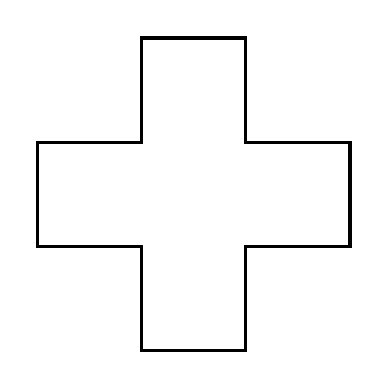
\includegraphics[width=3cm]{Argcrossscr}}{Cross}
Transform the script given below into a method named \ct{cross:} that draws a cross with the length of one of its 
arms passed as argument. You should then be able to execute the expression \ct{pica cross: 100.} Hint: notice 
that \ct{50 = 100 / 2}. A good name for the parameter might be \ct{armLength}. 

\ct{| pica |} \\
\ct{pica := Bot new.} \\
\ct{4 timesRepeat: }\\
    \ct{     [ pica go: 50.} \\
    \ct{     pica turnLeft: 90.} \\
    \ct{     pica go: 100.} \\
    \ct{     pica turnRight: 90.} \\
    \ct{     pica go: 100.}\\
    \ct{     pica turnRight: 90.}\\
    \ct{     pica go: 50 ]}
\end{exofigwithsizeandtitle}


\section{Variables in Methods}

Just as we have used variables in our scripts to give names to certain quantities, we can also 
use variables in methods for the same purpose. If we wanted to tell pica to draw a polygon 
with side length 100, we might come up with something like Script~\ref{scr:14-2}. Because the value of 
the angle that \ct{pica} has to turn through depends on the number of sides of the polygon, I have 
introduced the variables \ct{numberOfSides} and \ct{angle}. The number of sides is assigned a certain 
value (\ct{numberOfSides := 6} in our example), and then angle is assigned a value that is calculated 
in terms of the value of \ct{numberOfSides}. Now if we want to change the number of sides of the 
polygon from 6, as defined in the script, to any other value, we need to change only the value 
assigned to \ct{numberOfSides} in the third line of the script, and we don’t have to worry about the 
angle. 

\begin{script}[14-2]{Drawing a polygon in a script using variables. }
| pica numberOfSides angle | 
pica := Bot new. 
numberOfSides:= 6. 
angle := 360 / numberOfSides. 
numberOfSides timesRepeat: 
    [ pica go: 100. 
    pica turnLeft: angle ] 
\end{script}


To convert Script~\ref{scr:14-2} into a method, we can define a parameter for the number of sides. 
This is done in Method~\ref{mth:143}, which defines the method \ct{polygon100:} for drawing a polygon 
with an arbitrary number of sides, each side having a length of 100 pixels. 

\begin{method}[143]{Drawing a polygon in a method using a variable and a parameter }
polygon100: numberOfSides 
"Draws a polygon with an arbitrary number of sides; 
the length of each side is 100 pixels" 
   | angle | 
   angle := 360 / numberOfSides. 
   numberOfSides timesRepeat: 
       [ self go: 100. 
       self turnLeft: angle ]
\end{method}



This method has one argument, \ct{numberOfSides}, and one variable, angle. Both of them are 
used within the code of the method. Since \ct{numberOfSides} is a parameter, its value is specified 
in the argument of any message that invokes the method, for example, \ct{pica polygon100: 7} 
for a seven-sided regular polygon (heptagon). The \ct{variableangle} is initialized in the text of the 
method by setting it to the necessary angle, which depends on the value of the parameter at the 
time a message is sent (so it will be 360 / 7 in our example). For any value of \ct{numberOfSides}, the 
\ct{variableangle} will have the correct value for a regular polygon with that number of sides. 

Now that you have the method \ct{polygon100:}, you can use it to draw polygons, as shown in Script~\ref{scr:14-3}. 



\begin{script}[14-3]{Using the method \ct{polygon100:} to draw a heptagon and a pentagon.}
| pica berthe| 
berthe := Bot new. 
pica := Bot new. 
berthe polygon100: 5. 
pica polygon100: 7.  
\end{script}


\section{Experimenting with Multiple Arguments}

Why should we be limited to polygons with side length 100? Wouldn’t it be better to have a 
method that draws an arbitrary regular polygon, where both the number of sides and the side 
length are determined when the message is sent? For that, we would need two parameters: 
\ct{numberOfSides} \emph{and} \ct{sideLength}. So, how do we create a method having two parameters? You 
can create a method with two parameters by writing a method name with two colons and 
placing one argument name after each colon. 



\note{To define a method with multiple parameters,terminate each word in the method name (one word 
for each parameter) with a colon,and place each parameter after its corresponding word in the method 
name. The method named \ct{polygon:size:} requires two arguments. The definition of the method \ct{polygon: 
numberOfSides size: sizeValue} defines two parameters, \ct{numberOfSides} and \ct{sizeValue}. The first 
parameter represents, as its name implies, the number of sides. The second parameter is related to the size 
of the polygon. It will be explained following the definition of the method.}

The definition of the method \ct{polygon:size:} is shown as Method~\ref{mth:143}. After you have 
defined it, you can then simply send a message such as \ct{pica polygon: 7 size: 100}. 



\begin{method}[144]{Polygon}
polygon: numberOfSides size: sizeValue 
	"Draws a polygon with the number of sides and size to be specified" 
	| angle sideLength | 
	angle := 360 / numberOfSides. 
	sideLength := 4 * sizeValue / numberOfSides. 
	numberOfSides timesRepeat: 
		[ self go: sideLength. 
		self turnLeft: angle ] 
\end{method}




You may wonder why the parameter \ct{sizeValue} does not specify the side length of the 
polygon, but instead, I decided to define the side length (given by the variable \ct{sideLength} 
in the method) to be \ct{4 * sizeValue / numberOfSides}. In order to keep all polygons with the 
same \ct{sizeValue} approximately the same size, I made all polygons have their perimeters equal 
to the perimeter of a square with side length \ct{sizeValue}. The perimeter of such a square is \ct{4 * sizeValue}. The result is that by setting the variable \ct{sideLengthequal to 4 * sizeValue / numberOfSides}, when the robot draws \ct{numberOfSides} sides each of length \ct{sideLength}, it 
ends up walking a distance equal to the perimeter of a square with side length \ct{sizeValue}. 
Thus for example, any polygon drawn with its second argument 100 will have perimeter 400 
pixels, and so all the polygons will be displayed using about the same fraction of the screen. 

You may think that the name of the parameter \ct{numberOfSides} is a bit too long and 
cumbersome. However, it is a very good name for the parameter, because it can easily be 
understood by any person reading the method. As we already discussed in Chapter 9, it is 
quite important that your code should be readable, almost like a story, by anyone. And that 
includes you: the name of a variable or parameter that is unclear may well stump you when 
you look at your code several months after you wrote it. 


\begin{exonofig}
Define a method \ct{rectangleWidth:height:} that draws a rectangle with its width and height passed as arguments. 
\end{exonofig}


\begin{exonofig}
By slightly modifying the method \ct{cross:} that you wrote in Experiment 14-2, define a method \ct{crossWalk1:walk2:}  that can draw the stylized crosses shown in Figure~\ref{crosses}. Order the parameters so that a normal cross like the one  drawn by \ct{cross:} will have its first parameter equal to twice the second, and so will be drawn by expressions  such as \ct{pica crossWalk1: 60 walk2: 30}. 
\end{exonofig}

\begin{figure}
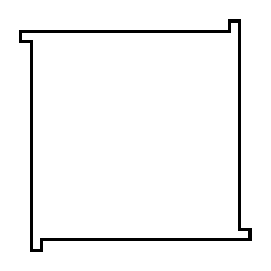
\includegraphics[width=3cm]{Argcrossscr2.pdf}\hfill
\includegraphics[width=3cm]{Argcrossscr3}\hfill
\includegraphics[width=3.8cm]{Argcrossscr4}
\caption{Three stylized crosses are produced by the method \ct{crossWalk1:walk2:}. The cross on 
the left is the result of the message send \ct{pica crossWalk1: 5 walk2: 50}; the middle cross is from 
\ct{pica crossWalk1: 50 walk2: 5}; the right-hand cross is from \ct{pica crossWalk1: 10 walk2: 20}. \label{crosses}}
\end{figure}

\section{Parameters and Variables }

Now that you have practiced a bit, it is time to look more carefully at the difference between 
ordinary variables and parameters. Let’s compare the script and method that were defined 
earlier for drawing a square of arbitrary side length. They are reproduced as Script~\ref{scr:14-4} and 
Method~\ref{mth:14-5}. 

In Script~\ref{scr:14-4}, first the variable \ct{sideLength} this declared (line 1), then a value is assigned to 
it (line 3), and finally it is used as the argument of the method \ct{go:} (line 5). 

\begin{script}[14-4]{}
(1)  | pica sideLength | 
(2)  pica := Bot new. 
(3)  sideLength := 10. 
(4)  4 timesRepeat: 
(5)       [ pica go: sideLength. 
(6)       pica turnLeft: 90 ] 
\end{script}


Method~\ref{mth:14-5} shows examples of two features of parameters. First, the parameter \ct{sideLength} is declared by being placed after a colon in the method name (line 1). Second, it is used 
as the argument of the message \ct{go:} (line 5). A parameter is not initialized in the method definition because it always gets its value from the corresponding argument in any message that 
invokes the method. For example, when the message \ct{pica square: 20} is sent to pica, then the 
parameter \ct{sideLength} of Method~\ref{mth:14-5} gets 20 as its value. 


\begin{method}[14-5]{The square-drawing method using a parameter}
(1) square: sideLength 
(2) "Draw a square of given side length" 
(3) 
(4) 4 timesRepeat: 
(5)      [ self go: sideLength. 
(6)      self turnLeft: 90 ] 
\end{method}

There are thus three distinctive differences between parameters and ordinary variables: 

\begin{description}
\item{\textbf{Parameters are not explicitly declared.}} Unlike other variables, a parameter does not 
have a variable declaration between vertical bars | |. A parameter is declared when it 
appears after a colon in the first line of the method’s definition. 

\item{\textit{Parameters cannot be assigned a value.}} Parameters cannot be modified the way other 
variables can. You cannot assign new values to parameters inside the body of a method 
definition. For example, in Method~\ref{mth:14-5} the expression \ct{sideLength := 100} is impossible. 
Parameters cannot have their values modified because they are a special kind of variable. 
They are placeholders for the arguments that are passed when a message invokes the corresponding method, and their values are assigned by Squeak when a message is sent and thus cannot be explicitly assigned using :=. 

\item{\textbf{Variable initialization.}} Ordinary variables and parameters get their values in very different 
ways. A variable value is changed by using an explicit assignment using :=. A parameter 
value is assigned when the method is invoked by a message. For example, the message 
send \ct{pica square: 10} causes the parameter \ct{sideLength} to be given the value 10. Thus a 
parameter is a variable, but it is a special type of variable whose value is assigned only at 
the time a message is sent and the corresponding method executed. 
\end{description}

\note{Aside from the three differences between parameters and ordinary variables,a parameter can be 
used in the code of a method definition just like any other variable. 
}




\section{Arguments and Parameters}

I have introduced the two terms \emph{argument} and \emph{parameter} for two related but different ideas. 
An argument is a specific object passed in a message. A parameter is the placeholder variable 
used in a method definition whose precise value isn’t known when the method is defined. 
A parameter takes its value from a corresponding argument.\footnote{Many authors define these terms differently. Some use “actual parameter” for what we call “argument” and “formal parameter” for what we call “parameter.” Others use the terms “parameter” and “argument” interchangeably.}

In Figure~\ref{fig:14-2}, in the message \ct{square: 100}, the number 100 is the message argument. 
When the method \ct{square:} is executed, its parameter \ct{sideLength} is set to 100, the value of the 
argument. 


\begin{figure}
	\begin{center}
\includegraphics[width=9cm]{argparam2}
\caption{The relationship between an argument (an object) and a parameter (a placeholder variable). \label{fig:14-2}}
\end{center}
\end{figure}


Another way to understand the difference between an argument and a parameter is that a 
parameter is a placeholder inside a method that represents an input to the method, while an 
argument is the actual value that is passed as this input. This idea is illustrated in Figure~\ref{fig:14-3}. 

\begin{figure}
	\begin{center}
\includegraphics[width=8cm]{argparam4}
\caption{The value of the argument is bound to the parameter during execution of the method. \label{fig:14-3}}
\end{center}
\end{figure}

Note that a parameter can also be used as an argument in other message sends. For 
example, in the definition of the method \ct{square:} (Method~\ref{mth:14-5}), the parameter \ct{sideLength} 
is used as the argument in the message \ct{go: sideLength}. 

A message argument can also be a variable. For example, in Script~\ref{scr:14-5}, which uses 
the method \ct{square:}, the argument of the first message square:is the value of the variable 
\ct{squareSize}, which is 100. The argument of the second message \ct{square:} is the value of the 
expression \ct{squareSize + 200}, which is 300. The parameter \ct{sideLength} of the method \ct{square:} 
gets the value 100 from the first \ct{square:} message, and then the value 300 from the second 
\ct{square:} message. 

\begin{script}[14-5]{A variable as argument}
| pica dist | 
pica := Bot new. 
squareSize := 100. 
pica square: squareSize. 
pica go: 300. 
pica square: squareSize + 200 
\end{script}

\section{About Method Execution}

On a first reading you may wish to skip this section, since it goes into details that beginners 
do not need to know. I wrote it because I wanted to answer the questions of the most curious 
readers, but I could as easily have omitted this paragraph without loss of continuity. 

When a method is executed, certain new variables are created. These variables are the 
message receiver selfand the method parameters (which refer to the method arguments), 
such as \ct{sideLength} in Figure 14-4, which shows the effect of sending the message square: 
length to a robot referred to by the variable pica, where the variable \ct{length} references the 
number 100.

\begin{figure}
	\begin{center}
\includegraphics[width=9cm]{argumentBoxes}
\caption{When a message is sent and a method executed,new variables are created that refer 
to the arguments and the receiver of the message.  \label{fig:14-4}}
\end{center}
\end{figure}






When the method \ct{square:} is executed, the variable \self refers to the message receiver, 
which in our example is the robot pointed to by the variable \ct{pica}; and the parameter \ct{sideLength} 
refers to the value of the variable length, which here is the number 100. The same process occurs 
for each message send. For example, the execution of the expression \ct{daly square: 200} assigns 
to \self the robot referenced by the variable \ct{daly} and assigns to \ct{sideLength} the number 200. 








This may look complex, but you do not have to worry about it. These are the hidden steps 
that Squeak takes to make sure that parameters are set to the values of the message arguments. 



\section{Summary} 

\begin{itemize}
	\item A parameter is a special kind of variable that acts as a placeholder for message arguments. A method parameter is declared right after a colon in the method name indicating the position of the parameter. A parameter must not be declared as a variable, and it cannot be assigned a value in the body of a method definition. Parameters receive their values from message arguments when a message invokes the method. 

	\item To define a method with multiple arguments, terminate each word in the method name 
with a colon, and place each parameter after its corresponding word in the method 
name. For example, the method named \ct{polygon:size:} requires two arguments. The 
definition of the method \ct{polygon: numberOfSides size: sizeValue} defines two 
parameters, \ct{numberOfSidesandsizeValue}. 

\end{itemize}

\ifx\wholebook\relax\else
    \end{document}
\fi


















\section{Other Graphical Patterns} 

In Chapter~\ref{cha:methods}, I asked you to define the method pattern, which draws a simple abstract pattern (See script~\ref{scr:125}). Now I will ask you to perform some further experiments that will 
produce more drawings by defining more methods. 

\begin{exofigwithsize}[0.5]{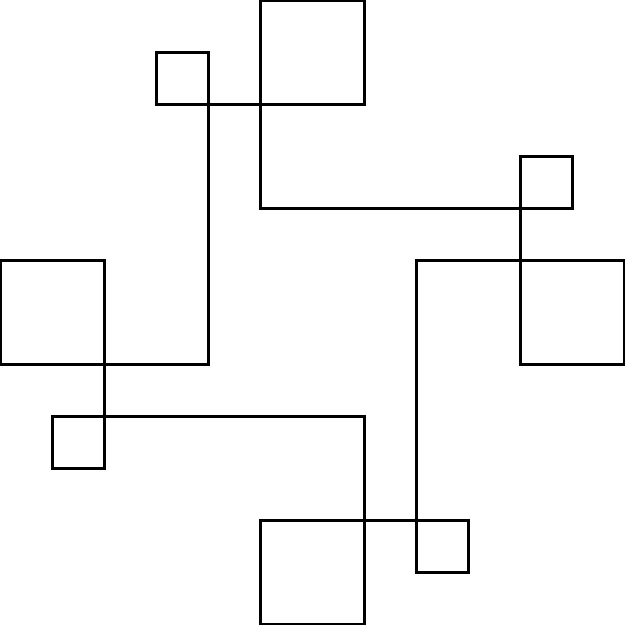
\includegraphics[width=5cm]{compCompleteThing}}{}\label{xp:131}
Define a method \ct{pattern4} that calls \ct{pattern} four times to produce the figure below. You will use this method 
later, in another script. After you have created the method \ct{pattern4}, use the following three-line script to make 
pica draw the figure.


\ct{| pica |} \\
\ct{pica := Bot new.} \\
\ct{pica pattern4 }

\end{exofigwithsize}


\begin{exonofigtitle}{A Ferris Wheel}
Define a method called \ct{tiltedPattern} that draws the picture at the beginning of this chapter, which looks 
somewhat like a Ferris wheel. Hint: you will have to call \ct{pattern} nine times, and the angle through which to turn 
between calls is 10 degrees. 
\end{exonofigtitle}


\begin{exofigwithsize}[0.5]{
\includegraphics[width=5cm]{compArtNouveauGiantScr}}{Doubling the Frame}\label{xp:133}
Define the method \ct{doubleFrame}, presented below,that draws the picture shown after the method definition. 


\textbf{doubleFrame}\\
\ct{8 timesRepeat:} \\
\ct{[ self pattern.} \\
\ct{self turnLeft: 45.} \\
\ct{self go: 100 ]} 
\end{exofigwithsize}



\begin{exonofigtitle}{Some Boxes}
Define methods boxandseparatedBoxthat produce the pictures shown in Figure~\ref{fig:131}. 
\end{exonofigtitle}


\begin{figure}[h]
	\centerline{\hfill\includegraphics[width=0.45\linewidth]{comp4Squares}\hfill
\includegraphics[width=0.45\linewidth]{comp4SquaresTwo}\hfill}
	\caption{Boxes
	\label{fig:131}}
\end{figure}


\begin{exonofigtitle}{Your Choice}
Use your previous methods to generate various figures of your choice.Have fun! 
\end{exonofigtitle}


\begin{exonofigtitle}{A Star}
Using the method \ct{box}, experiment and define a method \ct{star} that produces the right-hand picture in Figure~\ref{fig:132}.
\end{exonofigtitle}

\begin{figure}[h]
	\centerline{\hfill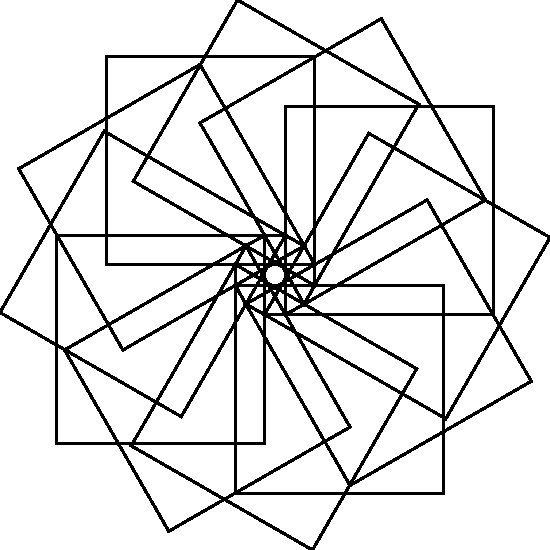
\includegraphics[width=0.45\linewidth]{comp4SquaresThree}\hfill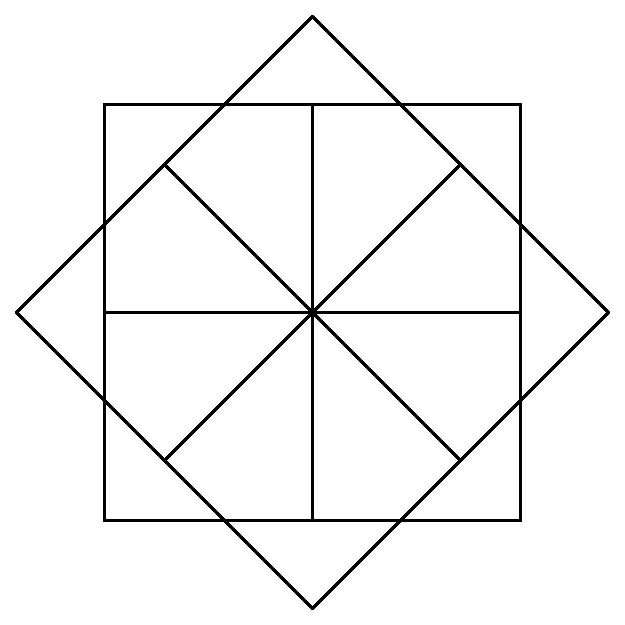
\includegraphics[width=0.45\linewidth]{comp4SquaresFour}\hfill}
	\caption{Stars
	\label{fig:132}}
\end{figure}



\ifx\wholebook\relax\else
    \end{document}
\fi

%%% Local Variables:
%%% coding: utf-8
%%% mode: latex
%%% TeX-master: t
%%% TeX-PDF-mode: t
%%% ispell-local-dictionary: "english"
%%% End:
